\documentclass[letterpaper, 10pt, conference]{ieeeconf}
\usepackage{times}

\IEEEoverridecommandlockouts
\overrideIEEEmargins

\let\proof\relax
\let\endproof\relax

\usepackage{amsmath, amssymb}
\usepackage{url}
\usepackage[pdftex]{graphicx}
\usepackage{float}
\usepackage{relsize}
\usepackage{algorithm}
\usepackage{fancyvrb}
\usepackage[noend]{algorithmic}
\usepackage{subfiles}
\usepackage{titlecaps}
\usepackage{fancyhdr}
\usepackage{amsthm}

\renewcommand{\thefootnote}{\fnsymbol{footnote}}
\renewcommand{\algorithmicrequire}{\textbf{Input:}}
\renewcommand{\algorithmicensure}{\textbf{Output:}}
\newcommand{\tab}[1]{\hspace{.2\textwidth}\rlap{#1}}
\newcommand{\itab}[1]{\hspace{0em}\rlap{#1}}
\renewcommand{\thefootnote}{\fnsymbol{footnote}}
\newcommand{\Acronym}[1]{\ensuremath{{{\texttt{#1}}}}}
\newcommand{\Symbol}[1]{\ensuremath{\mathcal{#1}}}
\newcommand{\Function}[1]{\ensuremath{{ \textsc{#1}}}}
\newcommand{\Constant}[1]{\ensuremath{{\texttt{#1}}}}
\newcommand{\Var}[1]{\ensuremath{{{\textsl{#1}}}}}
\newcommand{\False}{\Constant{false}}
\newcommand{\True}{\Constant{true}}
\newcommand{\Null}{\Constant{null}}
\newcommand{\dif}{\ensuremath{{\mathrm{d}}}}
\newcommand{\Name}{\Acronym{Dodger}}
\newcommand{\Revision}[1]{\textcolor{red}{#1}}
\newcommand{\R}{\ensuremath{\mathbb{R}}}
\newcommand{\Traj}{\ensuremath{\zeta}}
\newcommand{\Tree}{\Symbol{T}}
\newcommand{\pair}[1]{\ensuremath{\langle#1\rangle}}
\newcommand{\argmin}[1]{\underset{#1}{\operatorname{arg}\,\operatorname{min}}\;}
\newcommand{\argmax}[1]{\underset{#1}{\operatorname{arg}\,\operatorname{max}}\;}
\newcommand{\mychange}[1]{\textcolor{red}{#1}}

\begin{document}

\title{Developing Topological Representations for Robotic Exploration
    of Known Environments}


\author{Alex Wallar \and Donald A. Sofge \and Daniela Rus
\thanks{A. Wallar and D. Rus are with the Computer Science and Artificial
    Intelligence Laboratory at the Massachusetts Institute of Technology.
    D. Sofge is with the Naval Center for Applied Research in Artificial
    Intelligence at the Naval Research Laboratory}}

\maketitle

\begin{abstract}

    % In the domain of mobile robotics, the ability for a robot to navigate
    % safely through an uncertain dynamic environment is a core component of
    % autonomy.  In many situations, the motion of dynamic obstacles is
    % predictable. This information can be used by a planner to generate safe,
    % collision free paths to the goal. This paper develops a novel probabilistic
    % representation of dynamic obstacles using their predicted trajectories that
    % can account for an obstacle diverging from its prescribed path. This
    % representation is used to add time dependent costs on the edges of a
    % probabilistic roadmap (PRM). A graph search algorithm is presented that can
    % find safe paths through the PRM to guide a robot from its initial
    % configuration to a goal configuration amidst stochastic dynamic obstacles.
    % The developed planning approach is shown to outperform a potential fields
    % planner for guiding a robot in multiple situations and for different
    % notions safety.
    test

\end{abstract}

\section{Introduction}

In the context of mobile robotics, it is vital for a robot or a planner to
understand the topological and metric connectivity of the environment it is
operating in.  In order to conduct higher level planning such as monitoring
locations of interest or harvesting resources, a map of the environment is
needed that is able to represent through which paths two areas in the
environment are connected. There has been a lot of work in persistent coverage
and autonomous surveillance which solve variations of the travelling salesman
problem on graphical representations of an environment that assume knowledge of
the paths between areas of interest in their
search~\cite{yu2014correlated,sariel2009multiple,mitchell2015multi,
stump2011multi} but do not provide a method of determining these paths. This
work seeks to provide an simple graphical representation such that there are a
low number of nodes in the representation in order for solutions to the
travelling salesman problem and its variants are still feasible and a user of
the presented algorithm will be able to simply look-up the path between areas
of interest.

There has been a lot of work done in generating roadmaps of the environment
(i.e.\ graphs that represent the connectivity of the environment). Kavraki et
al developed the very popular probabilistic roadmap which randomly samples
points in the configuration space of a robot and connects them in a graphical
structure if it is feasible for the robot to move from one configuration two
another avoiding collisions~\cite{prm}. LaValle developed the rapidly-exploring
random tree which incrementally develops a tree like structure of paths that
would lead a robot from an initial to a goal configuration~\cite{rrt}. However,
these approaches do not provide a concise graphical representation of the
environment.

There has also been a lot of work in thinning free space to provide a more
concise representation. Beenson et al developed a topological thinning
algorithm using an Extended Voronoi Graph (EVG) that can show topologically
distinct paths in free space~\cite{evg}. However, the work lacks a concise
graphical structure.  Instead of providing a graph representing the
connectivity, the work has provided a list of points which lie on the thinned
representation of free space. Similarly, work has been done using morphology
operations to produce a thin skeleton of the original
volume~\cite{graphicsGems,skeletonize3d} but do not provide information about
the connectivity of regions. Portugal and Rocha were able to use the work done
by Beenson et al to determine the location of critical points that can be used
as nodes in a graph~\cite{david}, however this work did not provide a means of
determining edges between the discovered nodes.

This paper presents an algorithm that is able to provide a graphical structure
that represents both the topological and metric connectivity of the environment
with a smaller number of nodes than work done previously by Portugal and Rocha
and a simple look-up procedure to determine the path between nodes. Our method
consists of three steps:

\begin{enumerate}
    \item Produce a Voronoi graph of the environment using boundary points
        along the obstacles as centers of the Voronoi cells
    \item Reduce the number of nodes by pruning redundant nodes that are not
        critical in defining the topological or metric connectivity of the
        environment
    \item Prune the redundant leaf branches left over from the Voronoi
        graph
\end{enumerate}

These steps are discussed in more detail in sections~\ref{sec:voronoi},
\ref{sec:prune_nodes}, and \ref{sec:prune_branches} respectively.


\section{Developing the Initial Voronoi Diagram}

\label{sec:voronoi}

We develop the initial graphical representation of the environment by
determining points along the edge of all the obstacles in the environment. We
use these points as centers of the Voronoi cells and provide them to the
Voronoi diagram algorithm to determine the initial topological representation.
This is the technique used by Choset and Burdick when developing generalized
Voronoi graphs of occupancy grids~\cite{choset2000sensor}.
Algo.~\ref{algo:boundary} shows how these boundary points are chosen from the
occupancy grid.

In order to extract a graphical structure from the Voronoi diagram, the points
along the ridges are used as vertices. The vertices are connected to other
points along the same ridge. Ridges that intersect obstacles and ridges totally
contained by obstacles are discarded. This connected structure provides the
first graphical representation of the environment.

% \begin{figure}[h!]
%     \centering
%     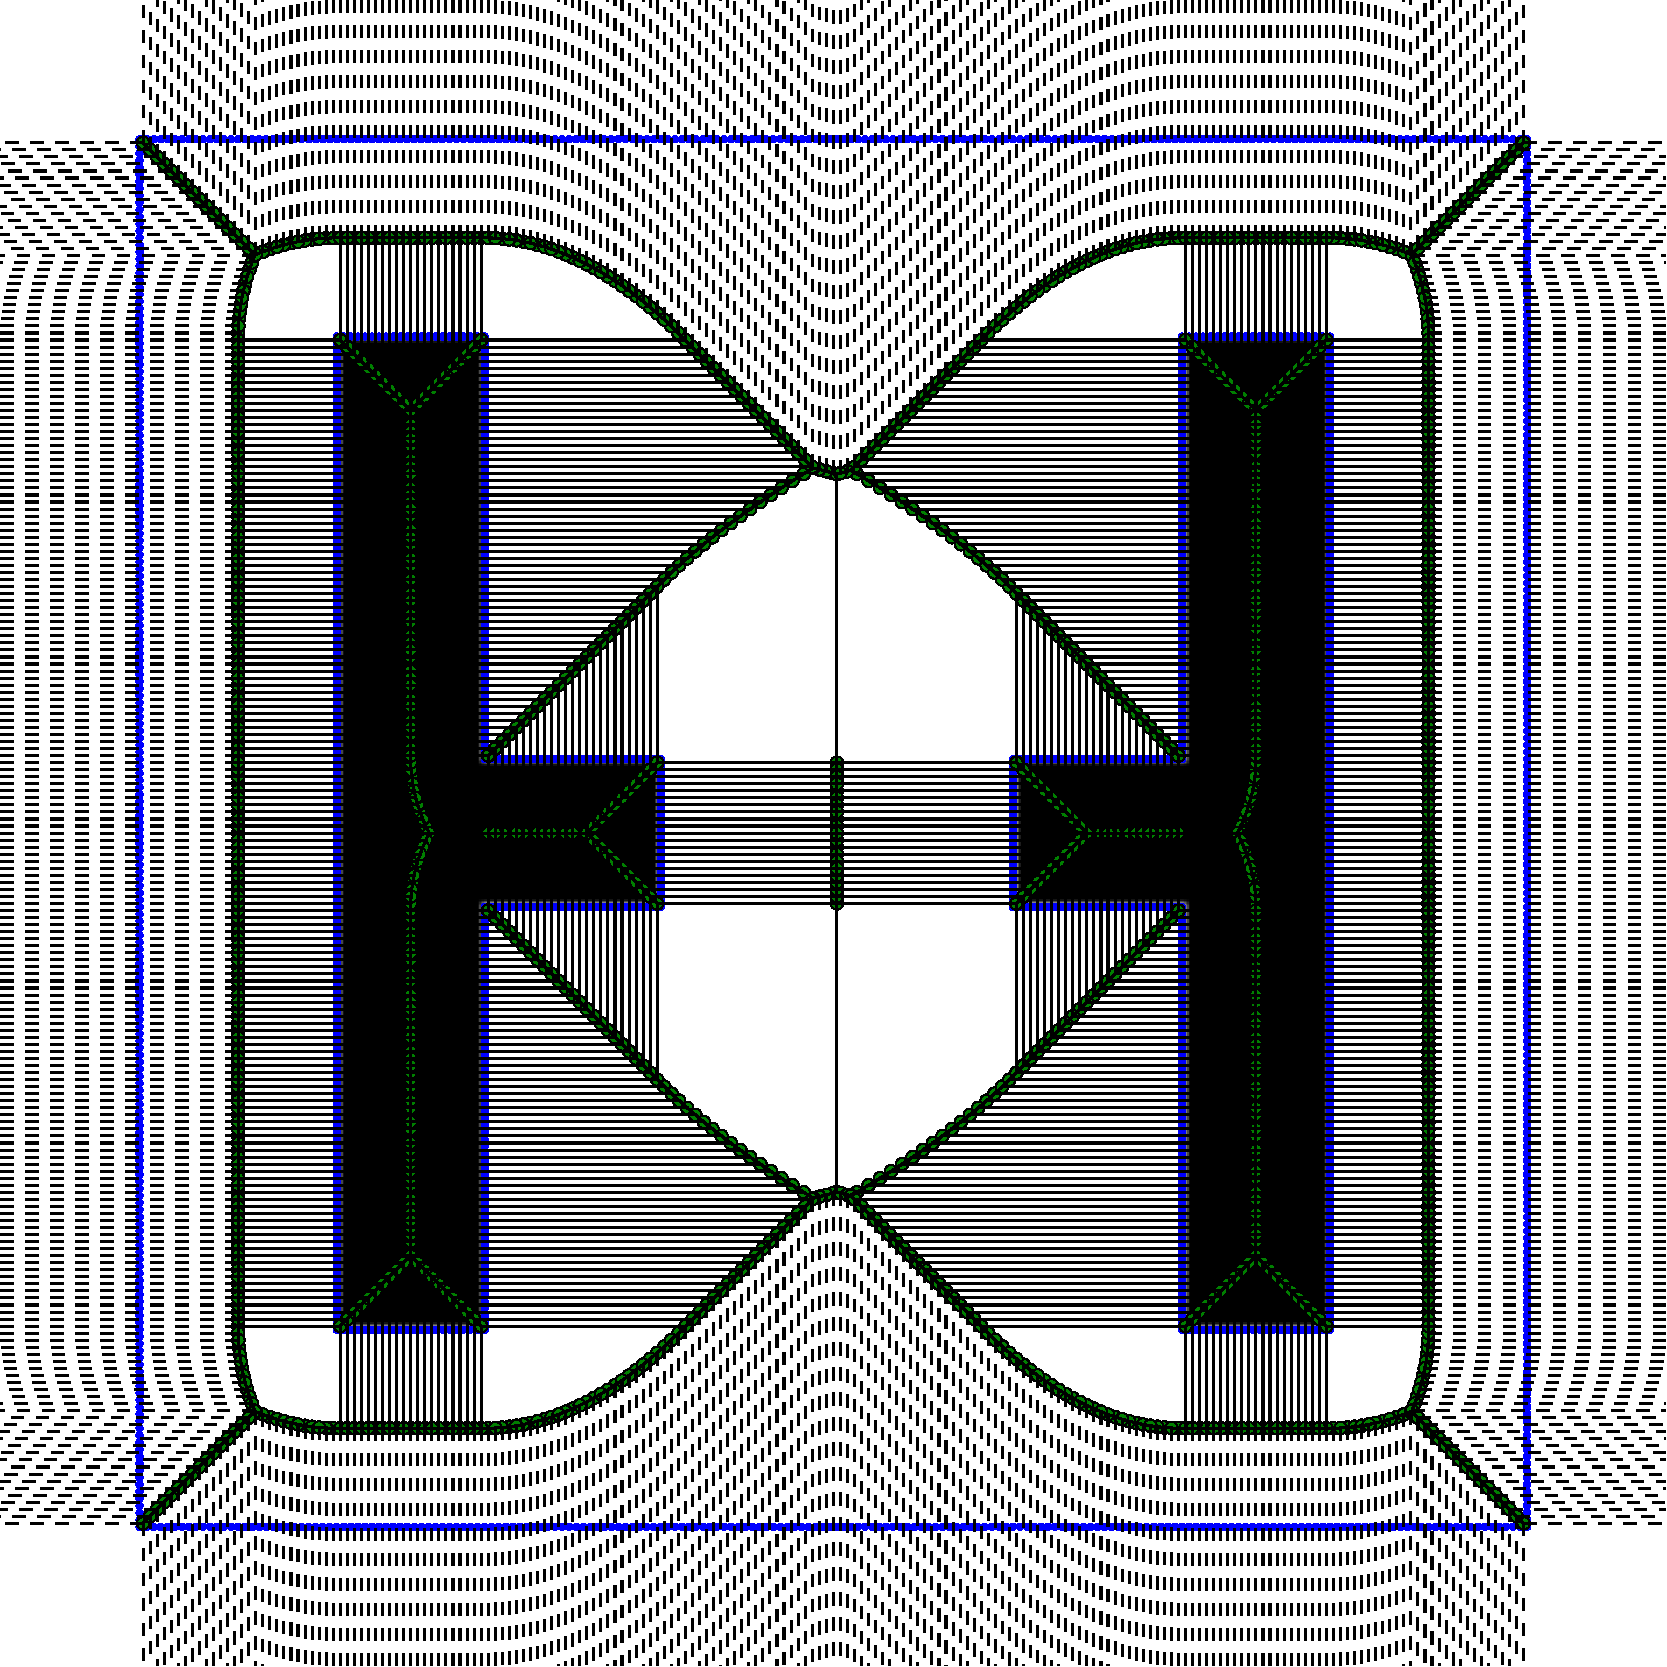
\includegraphics[width=1\linewidth]{figs/initial_vor}
% \end{figure}

\begin{algorithm}[h!]
    \caption{$\Function{BoundaryPoints}(\mathcal{O})$}
    \algorithmicrequire{
        \begin{itemize}
            \item $\mathcal{O}$: $M \times N$ binary matrix representing
                obstacles in the environment, where if $\mathcal{O}_{i, j}$ is
                $1$, $(i, j)$ is inside an obstacle
        \end{itemize}}
    \algorithmicensure{
        \begin{itemize}
            \item A set of pairs representing boundary points in the
                occupancy grid
        \end{itemize}}

    \label{algo:boundary}
    \begin{algorithmic}[1]
        \setcounter{ALC@line}{0}
        \vspace*{1mm}
        \STATE $S \leftarrow \{\}$
        \FOR{$i = 1$ \TO $M$}
            \FOR{$j = 1$ \TO $N$}
                \IF {$\mathcal{O}_{i, j} = 1$}
                    \FOR{$k = -1$ \TO $1$}
                        \FOR{$l = -1$ \TO $1$}
                            \IF{$\mathcal{O}_{i + k, j + l} == 0$}
                                \STATE $S \leftarrow S \cup \{(i, j)\}$
                            \ENDIF
                        \ENDFOR
                    \ENDFOR
                \ENDIF
            \ENDFOR
        \ENDFOR
        \RETURN $S$
    \end{algorithmic}
\end{algorithm}

\section{Pruning Redundant Nodes}

\label{sec:prune_nodes}

In order to produce a graph with a relatively small number of vertices, we need
to prune vertices from the graph generated by the Voronoi diagram that are not
critical to defining the metric and topological structure of the environment. A
critical node is defined as any node with one edge or with three or more edges.
The initial pruning of redundant nodes is done by first determining which nodes
in the original graph are critical and connecting them through a series a of
non-critical points.  This chain of non-critical points will develop the path
between the critical nodes.  After pruning these nodes, a directed multi-graph
structure, $G = (V, E, \Pi)$, which contains a set of critical nodes, a set of
pairs representing the topological connectivity between nodes, and a set of
sequences representing the geometric paths between the nodes is produced. Note
that this graph structure is able to have multiple paths between the same pair
of nodes.

To develop this initial reduced graph, we iterate through all of the critical
nodes in the original graph determined by the Voronoi diagram. Then for each
neighbour of each critical node, we determine if that node is also critical. If
so, an edge is created and the iteratively stored path between them is added to
the edge. If the neighbour is not a critical node, it gets added to path
stemming from the critical node until another critical node is discovered. This
process is shown in Algo.~\ref{algo:rtvd}.

\begin{algorithm}[h!]
    \caption{$\Function{rTVD}(\mathcal{O})$}
    \algorithmicrequire{
        \begin{itemize}
            \item $\mathcal{O}$: $M \times N$ binary matrix representing
                obstacles in the environment
        \end{itemize}}
    \algorithmicensure{
        \begin{itemize}
            \item A graph representing the topological connectivity of the
                environment, $\mathcal{O}$, with redundant leaf branches.
        \end{itemize}}

    \label{algo:rtvd}
    \begin{algorithmic}[1]
        \setcounter{ALC@line}{0}
        \vspace*{1mm}
        \STATE $P \leftarrow \Function{BoundaryPoints}(\mathcal{O})$
        \STATE $\mathcal{V} \leftarrow \Function{Voronoi}(P)$
        \STATE $G = (V, E) \leftarrow \Function{DiGraph}()$
        \FOR{$i \in \Function{CriticalNodes}(\mathcal{V})$}
            \FOR {$j \in \Function{Neighbours}(i)$}
                \STATE $\Pi \leftarrow \{i\}$
                \STATE $S \leftarrow \{j\}$
                \WHILE {$|S| > 0$}
                    \STATE $n \leftarrow \Function{Pop}(S)$
                    \STATE $\Pi \leftarrow \Pi \cup \{n\}$
                    \IF {$n \in \Function{CriticalNodes}(\mathcal{V})$}
                        \STATE $V \leftarrow V \cup i$
                        \STATE $E \leftarrow E \cup (i, n, \Pi)$
                        \STATE \textbf{break}
                    \ELSE
                        \FOR{$m \in \Function{Neighbours}(n)$}
                            \IF{$m \notin \Pi$}
                                \STATE $S \leftarrow S \cup \{m\}$
                            \ENDIF
                        \ENDFOR
                    \ENDIF
                \ENDWHILE
            \ENDFOR
        \ENDFOR
        \RETURN $H$
    \end{algorithmic}
\end{algorithm}

\section{Pruning Redundant Leaf Branches}

\label{sec:prune_branches}

Once redundant nodes have been initially pruned from the Voronoi graph, we need
to remove leaf branches that have been generated which do not actually provide
any additional information about the environment. A heuristic is used to prune
these branches from the Voronoi graph. If a node has only one edge and it is
within a certain distance from any obstacle, it is removed from the graph. Once
leaf branches meeting this criteria are removed, we traverse the resulting
graph and remove nodes that have become redundant and are no longer critical
(i.e.\ they only have two edges). This is done by iterating through all of the
current critical nodes and traversing their neighbours. If the neighbour is not
critical, the node itself and the path connecting the critical node to the
neighbour are stored as the current path and all of it's neighbours are added
to the search. Once another critical node is reached, an edge is created
between them and the accumulated path is stored in the graphical structure.
This is shown more formally in Algo.~\ref{algo:tvd}. It is necessary to remove
these redundant leaf branches to provide a more concise representation of the
environment and reduce the number of nodes generated.
Fig.~\ref{fig:redundant_leaves} shows where redundant leaf branches are
generated and provides a motivation for their removal.

\begin{figure}[h!]
    \centering
    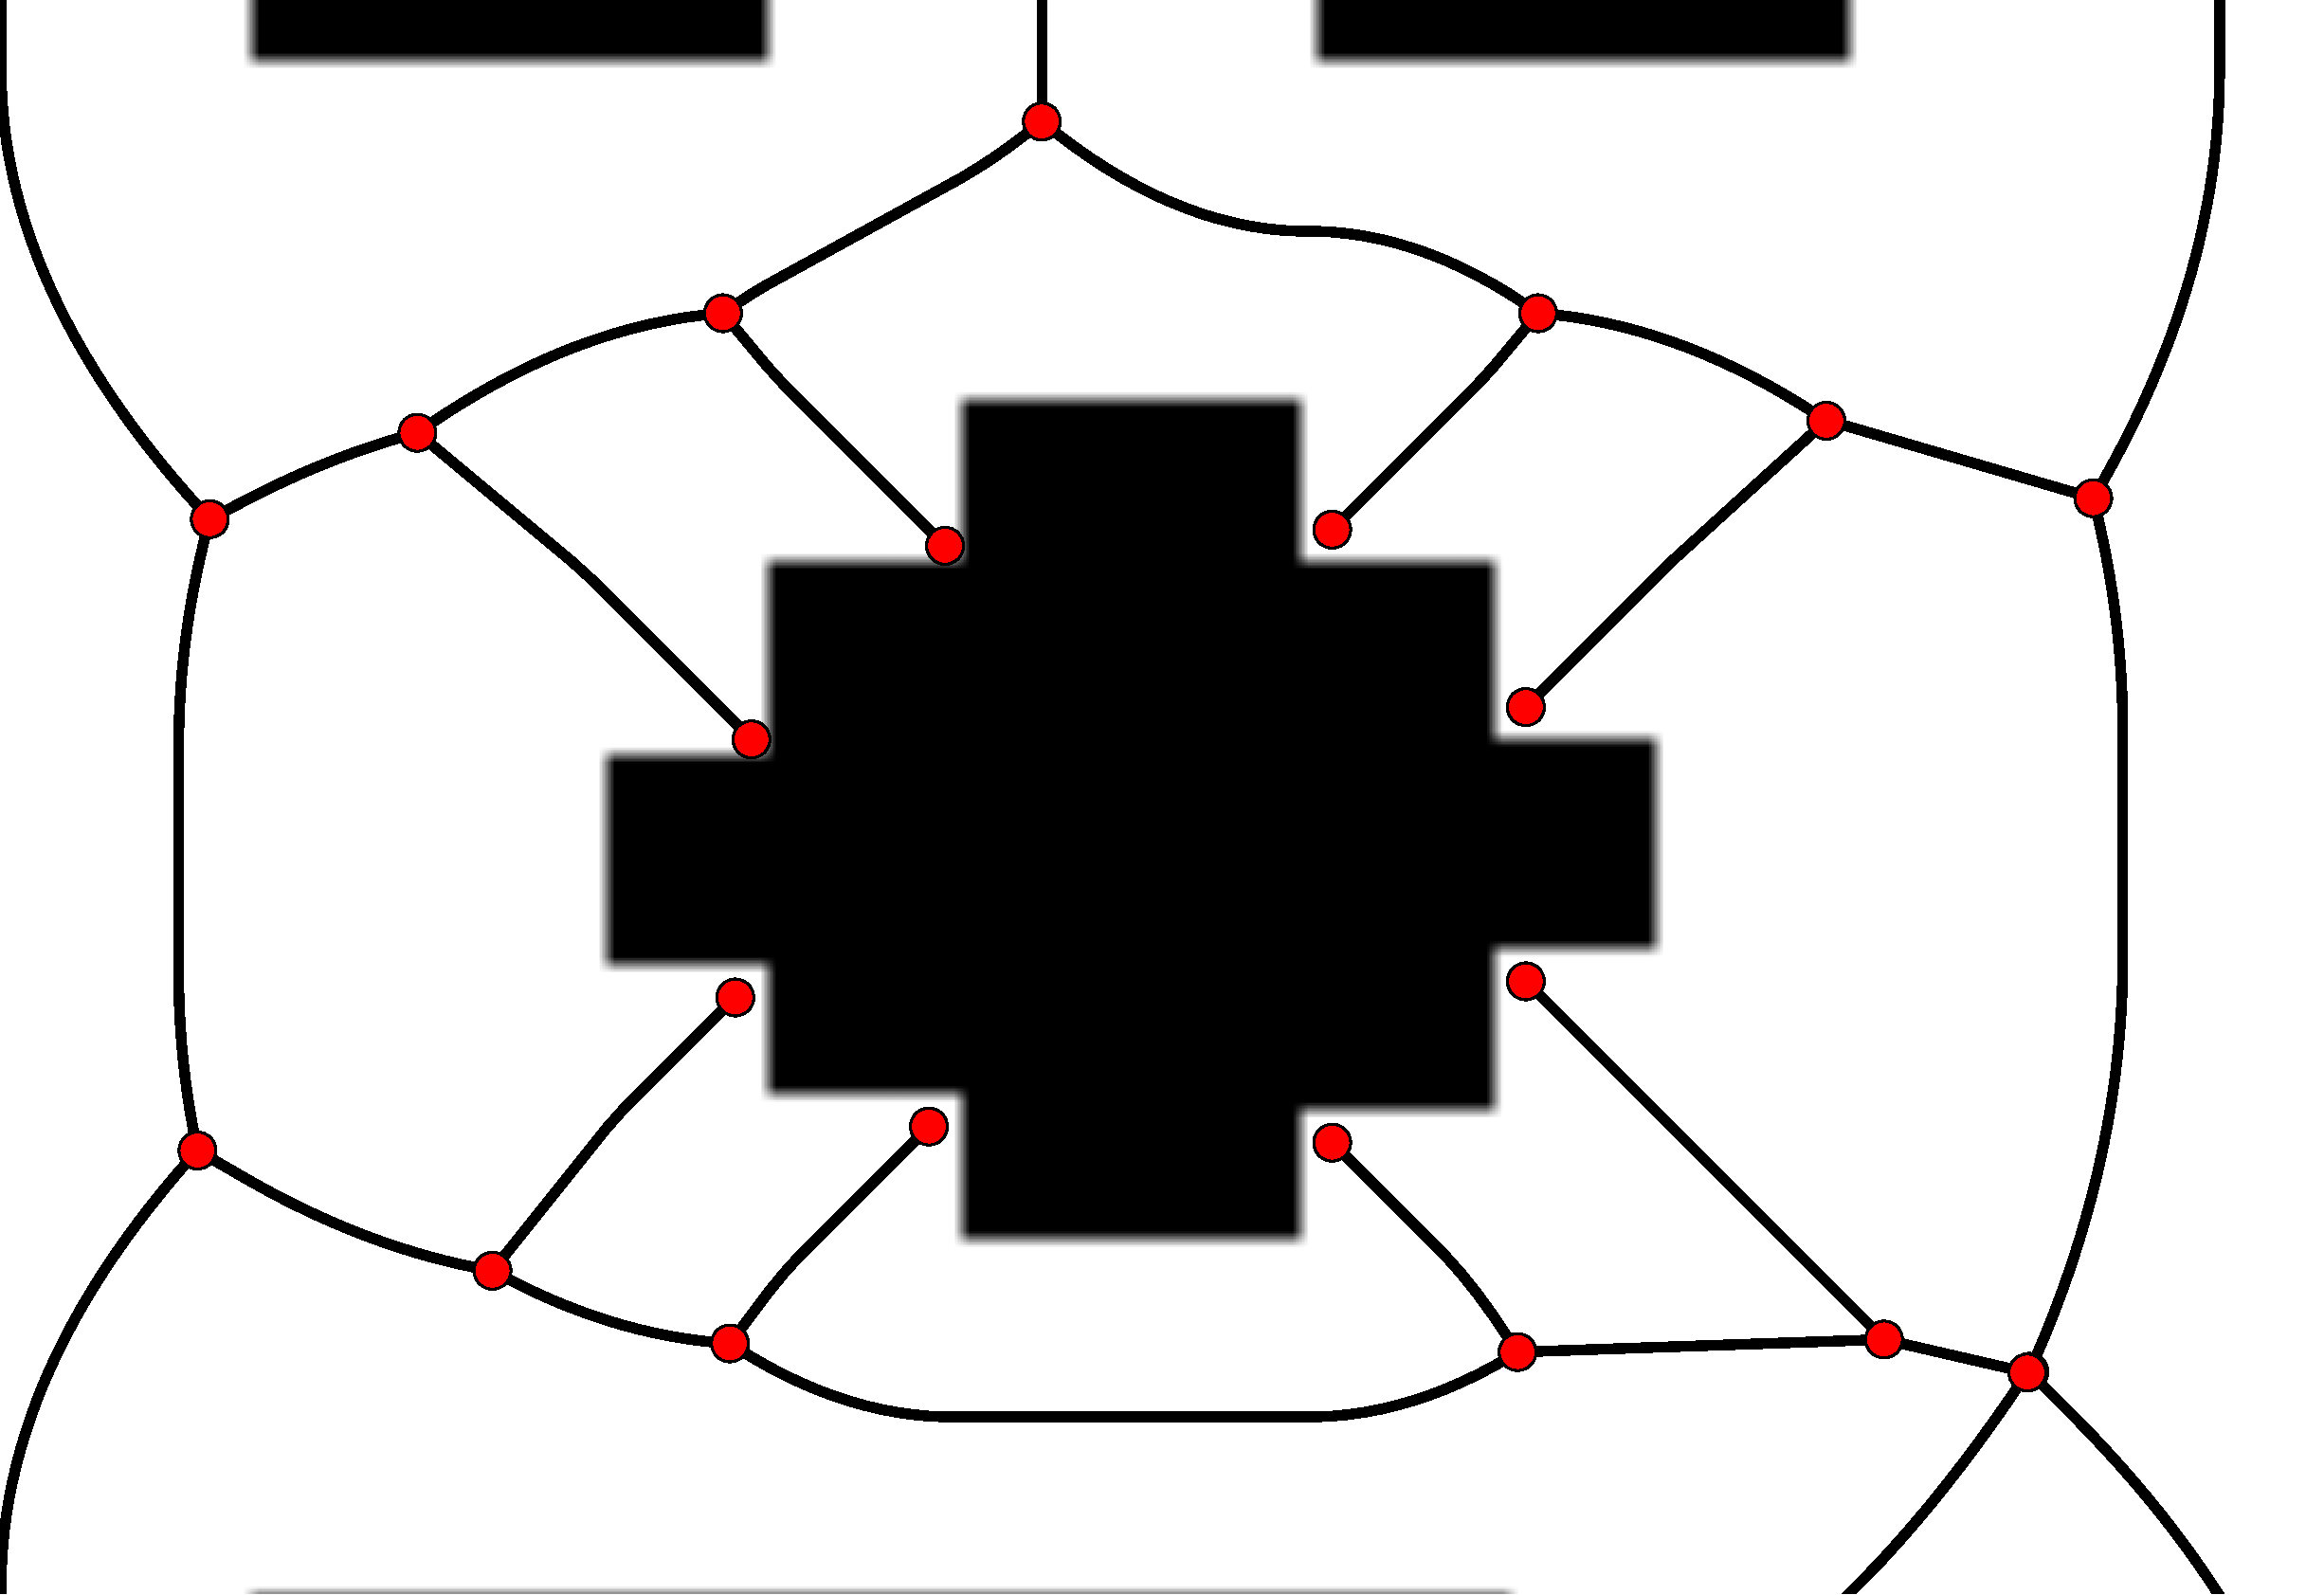
\includegraphics[width=1\linewidth]{figs/redundant_leaves_strongly_connected}
    \label{fig:redundant_leaves}
    \caption{Redundant leaves generated by the Voronoi diagram which are pruned
        by the propsed algorithm}
\end{figure}

\begin{algorithm}[h!]
    \caption{$\Function{TVD}(\mathcal{O})$}
    \algorithmicrequire{
        \begin{itemize}
            \item $\mathcal{O}$: $M \times N$ binary matrix representing
                obstacles in the environment
        \end{itemize}}
    \algorithmicensure{
        \begin{itemize}
            \item A graph representing the topological connectivity of the
                environment, $\mathcal{O}$
        \end{itemize}}

    \label{algo:tvd}
    \begin{algorithmic}[1]
        \setcounter{ALC@line}{0}
        \vspace*{1mm}
        \STATE $G = (V, E) \leftarrow \Function{MultiDiGraph}()$
        \STATE $H \leftarrow \Function{rTVD}(\mathcal{O})$
        \STATE $H' \leftarrow \Function{RemoveCloseNodes}(H, \mathcal{O})$
        \FOR{$i \in \Function{CriticalNodes}(H')$}
            \FOR {$j \in \Function{Neighbours}(i)$}
                \STATE $\Pi \leftarrow \{i\}$
                \STATE $S \leftarrow \{(i, j)\}$
                \WHILE {$|S| > 0$}
                    \STATE $(n, m) \leftarrow \Function{Pop}(S)$
                    \STATE $\Pi \leftarrow \Pi \cup \Pi_{H'}(n, m)$
                    \IF {$n \in \Function{CriticalNodes}(H')$}
                        \STATE $V \leftarrow V \cup i$
                        \STATE $E \leftarrow E \cup (i, n, \Pi)$
                        \STATE \textbf{break}
                    \ELSE
                        \FOR{$k \in \Function{Neighbours}(n)$}
                            \IF{$k \notin \Pi$}
                                \STATE $S \leftarrow S \cup \{(n, k)\}$
                            \ENDIF
                        \ENDFOR
                    \ENDIF
                \ENDWHILE
            \ENDFOR
        \ENDFOR
        \RETURN $G$
    \end{algorithmic}
\end{algorithm}

\begin{figure*}
    \centering
    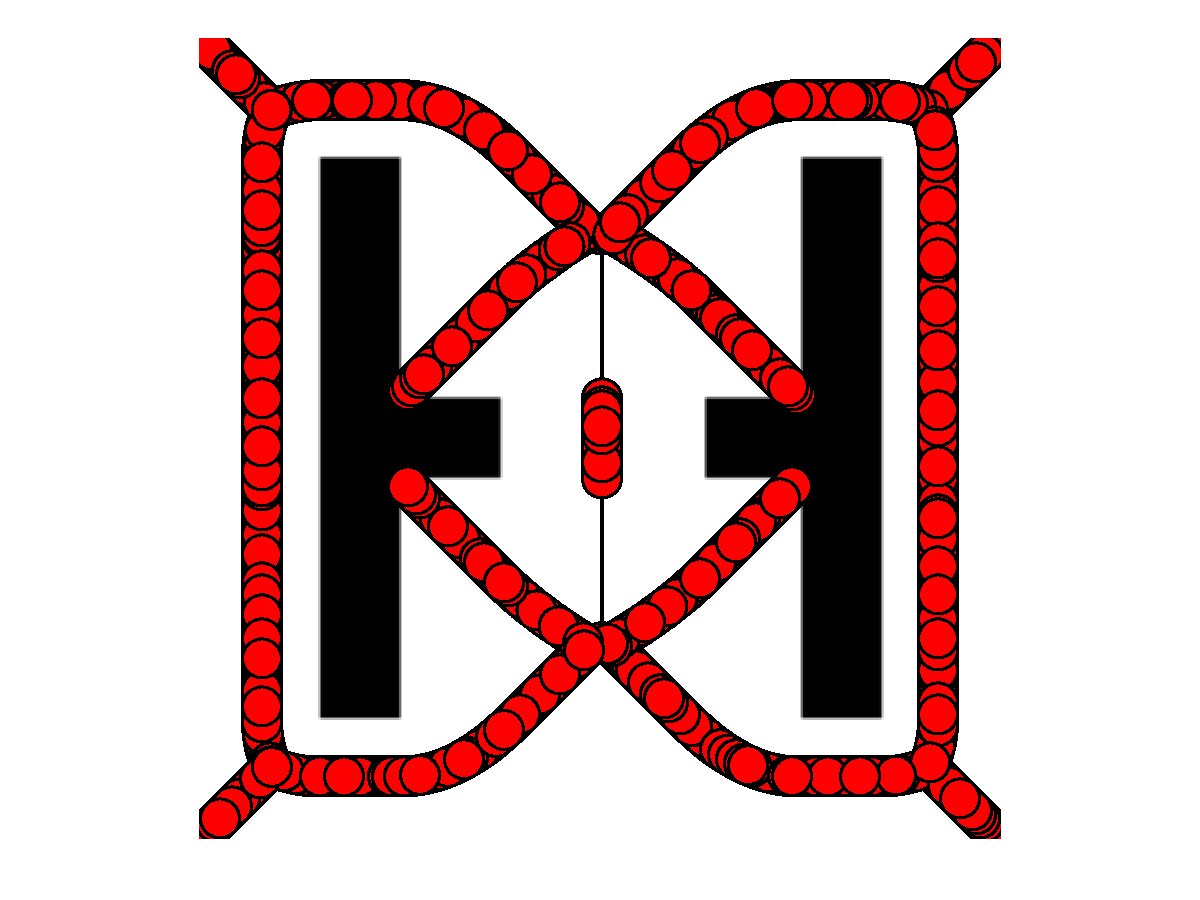
\includegraphics[width=0.32\linewidth]{figs/bars_vor}
    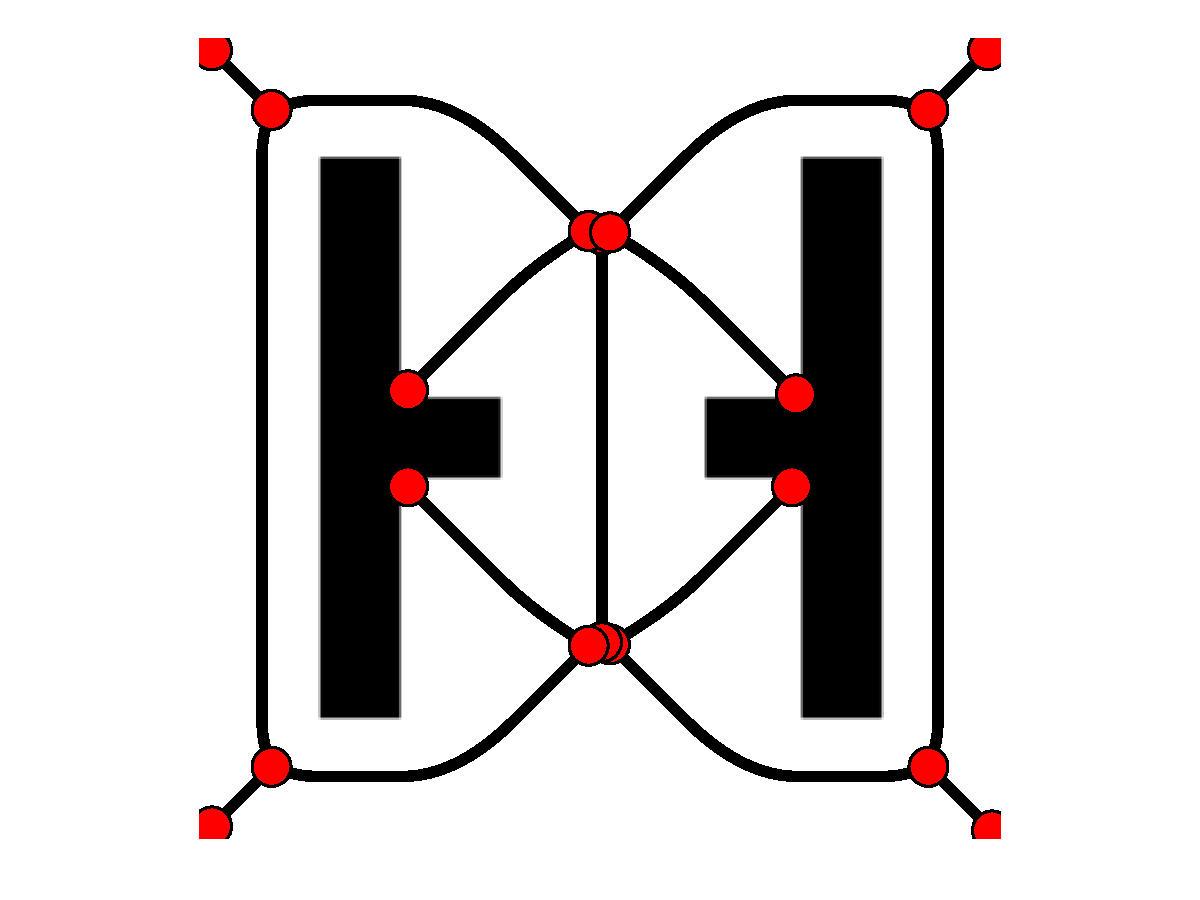
\includegraphics[width=0.32\linewidth]{figs/bars_leaves}
    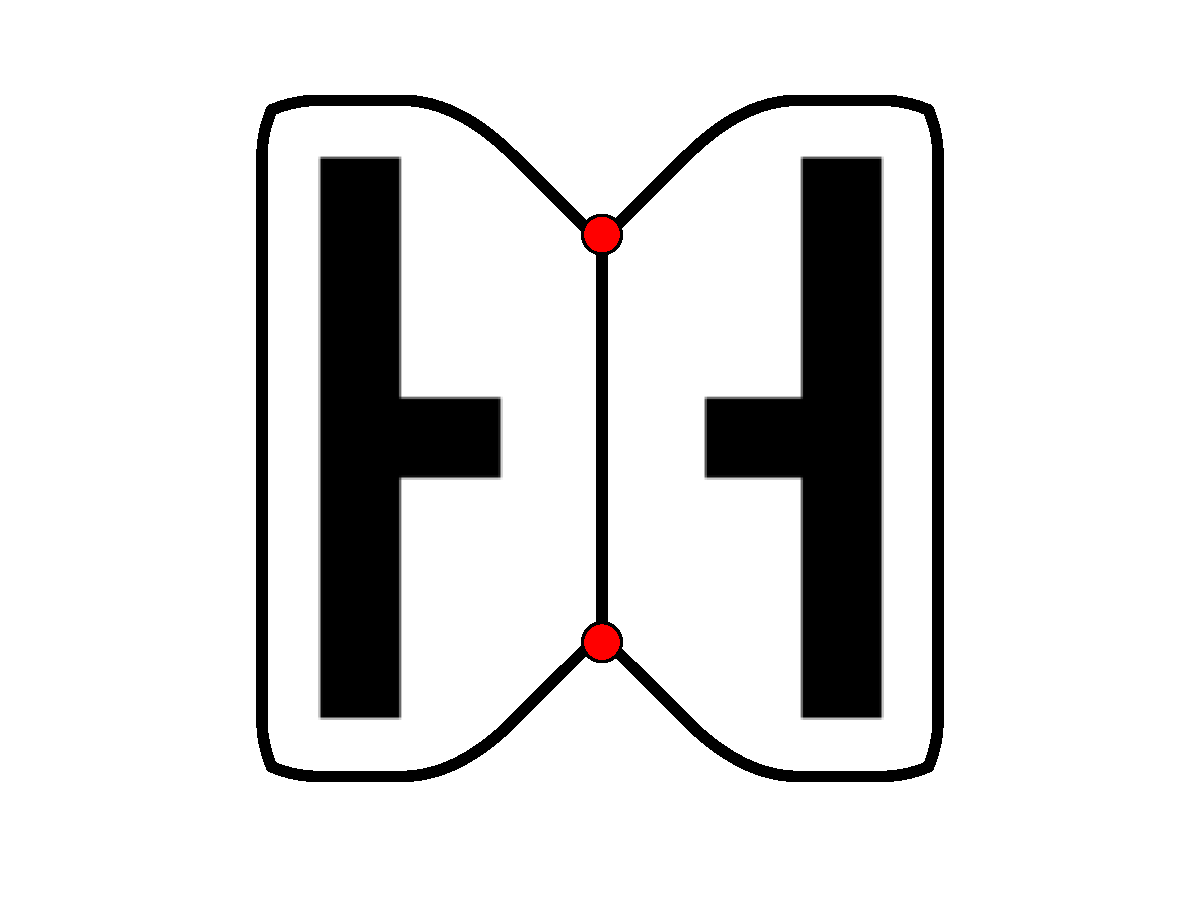
\includegraphics[width=0.32\linewidth]{figs/bars_TVD}\\
    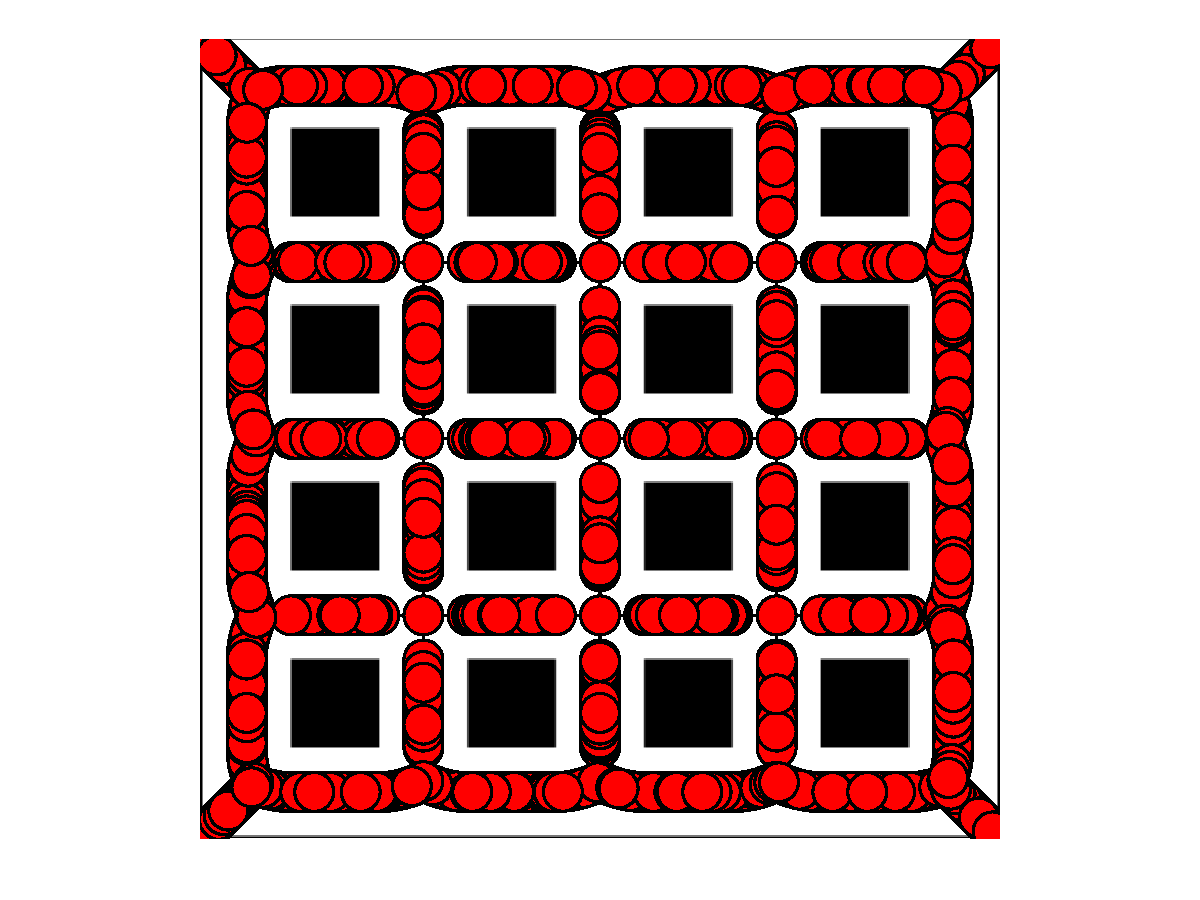
\includegraphics[width=0.32\linewidth]{figs/Grelha4_vor}
    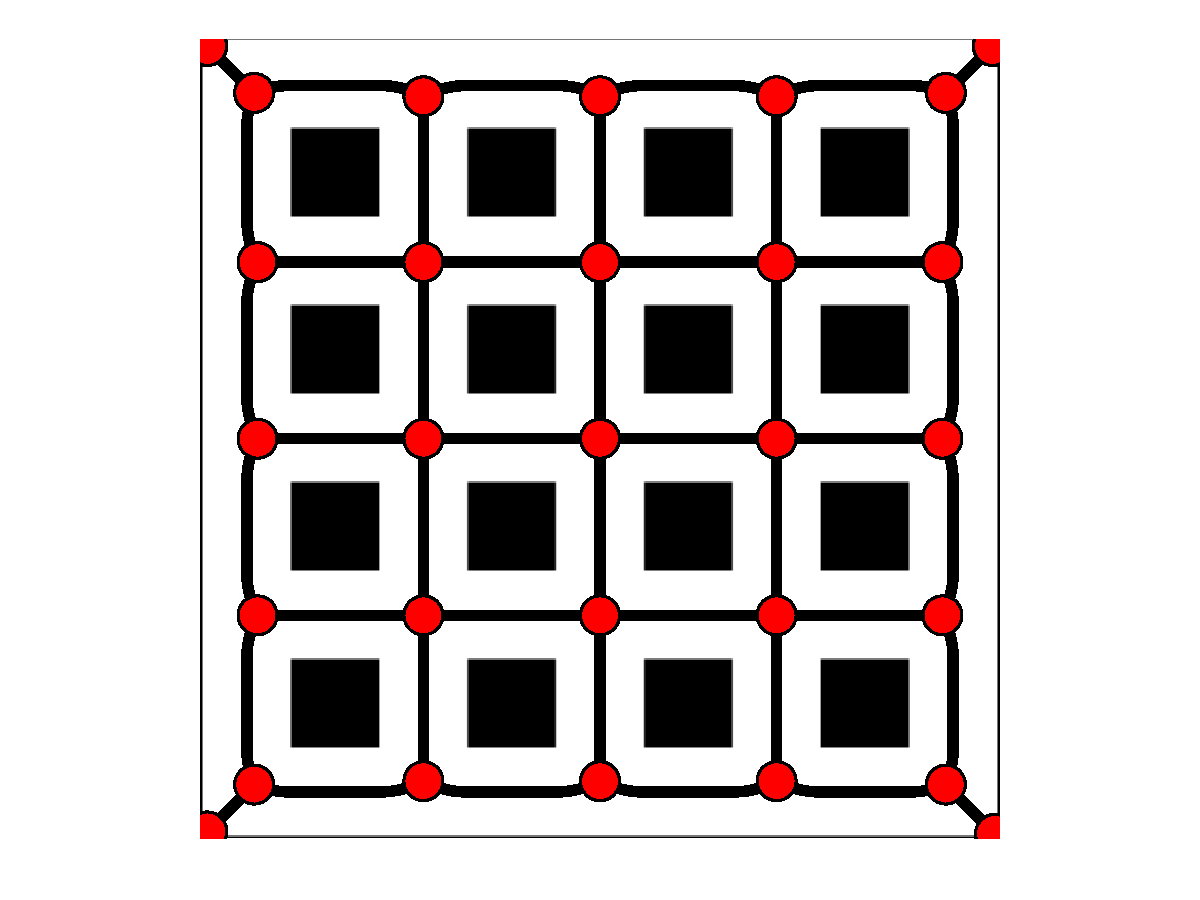
\includegraphics[width=0.32\linewidth]{figs/Grelha4_leaves}
    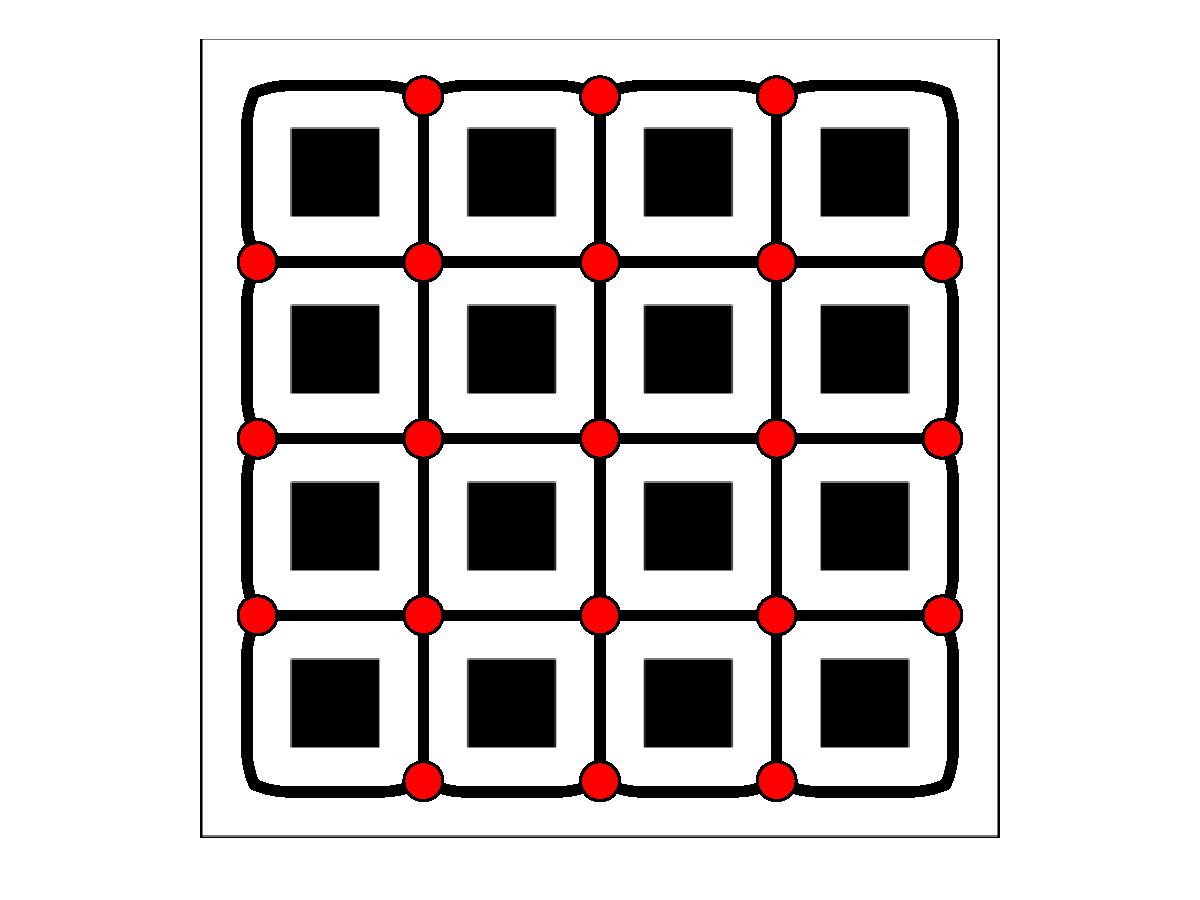
\includegraphics[width=0.32\linewidth]{figs/Grelha4_TVD}\\
    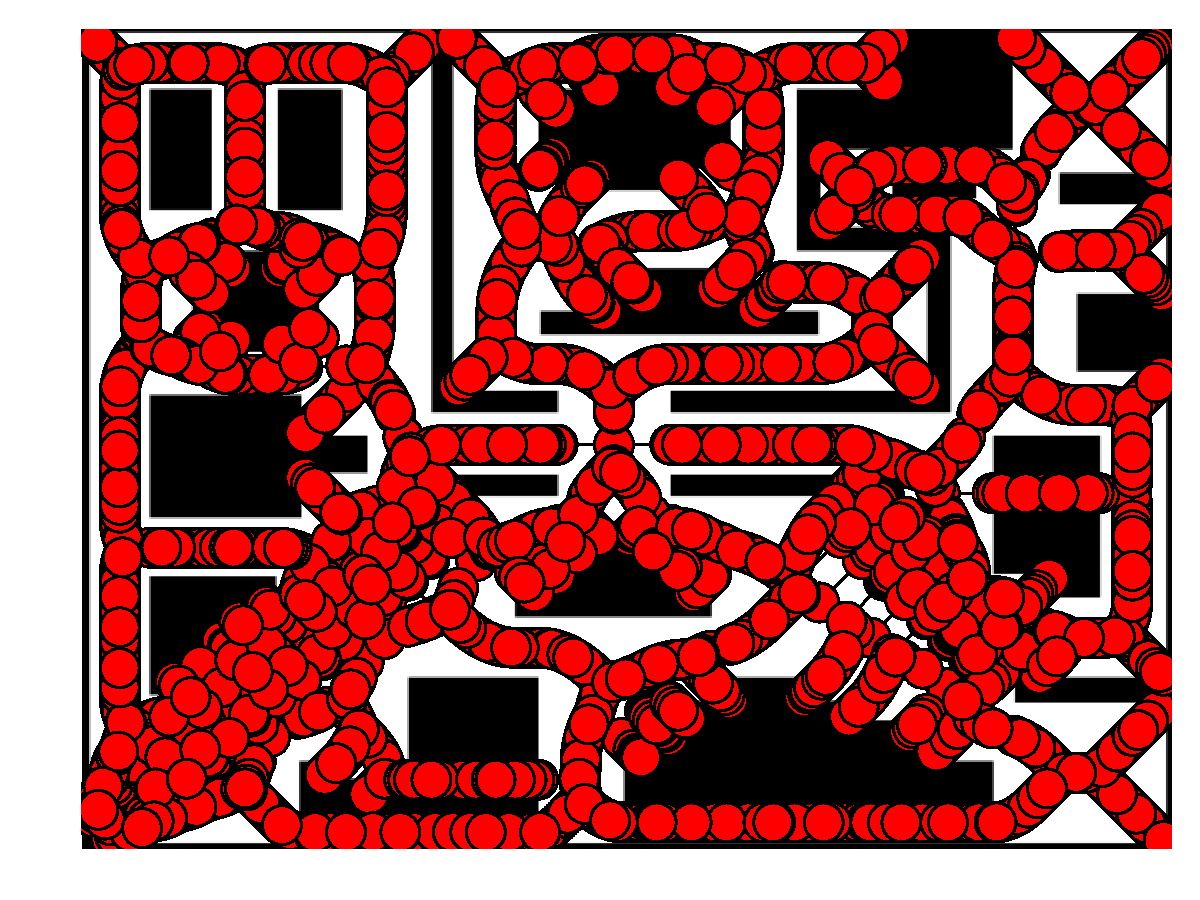
\includegraphics[width=0.32\linewidth]{figs/strongly_connected_vor}
    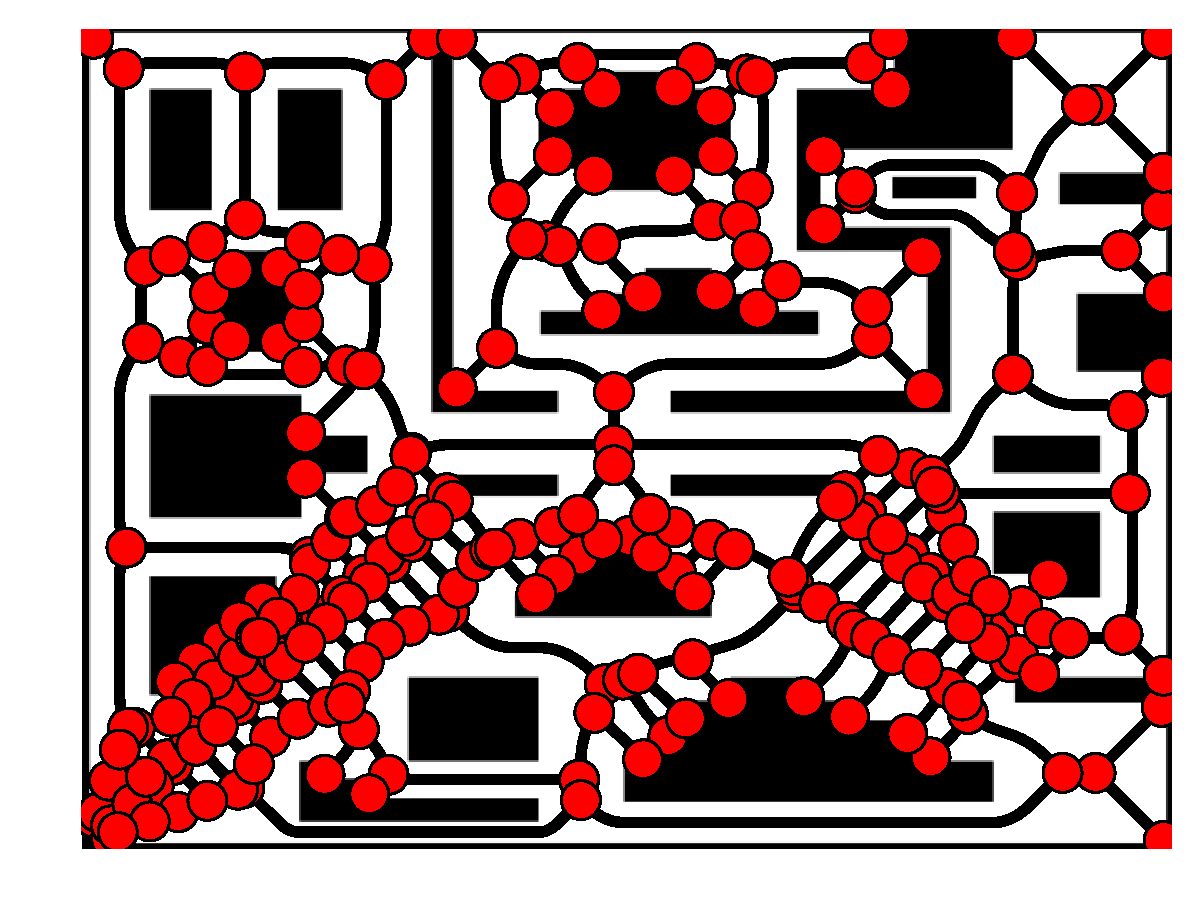
\includegraphics[width=0.32\linewidth]{figs/strongly_connected_leaves}
    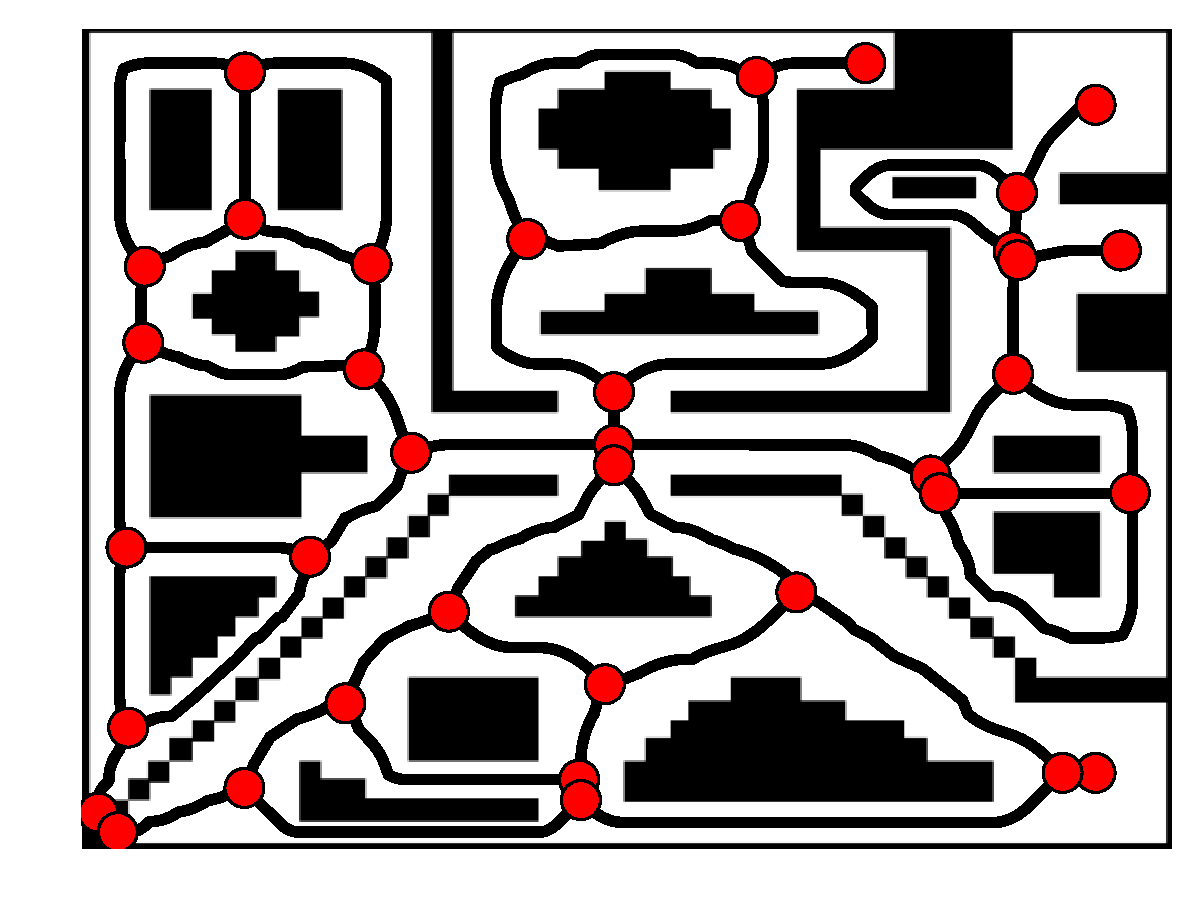
\includegraphics[width=0.32\linewidth]{figs/strongly_connected_TVD}

    \label{fig:process}
    \caption{The topological extraction algorithm running on each of the
        three scenes presented. The first column represents the graph generated
        from the initial Voronoi decomposition. The second column is a result
        of the first node reduction using $\Function{rTVD}$ and the last column
        is the final graph representing the connectivity of the environment
    generated by the second node reduction using $\Function{TVD}$.}
\end{figure*}

\begin{figure*}
    \centering
    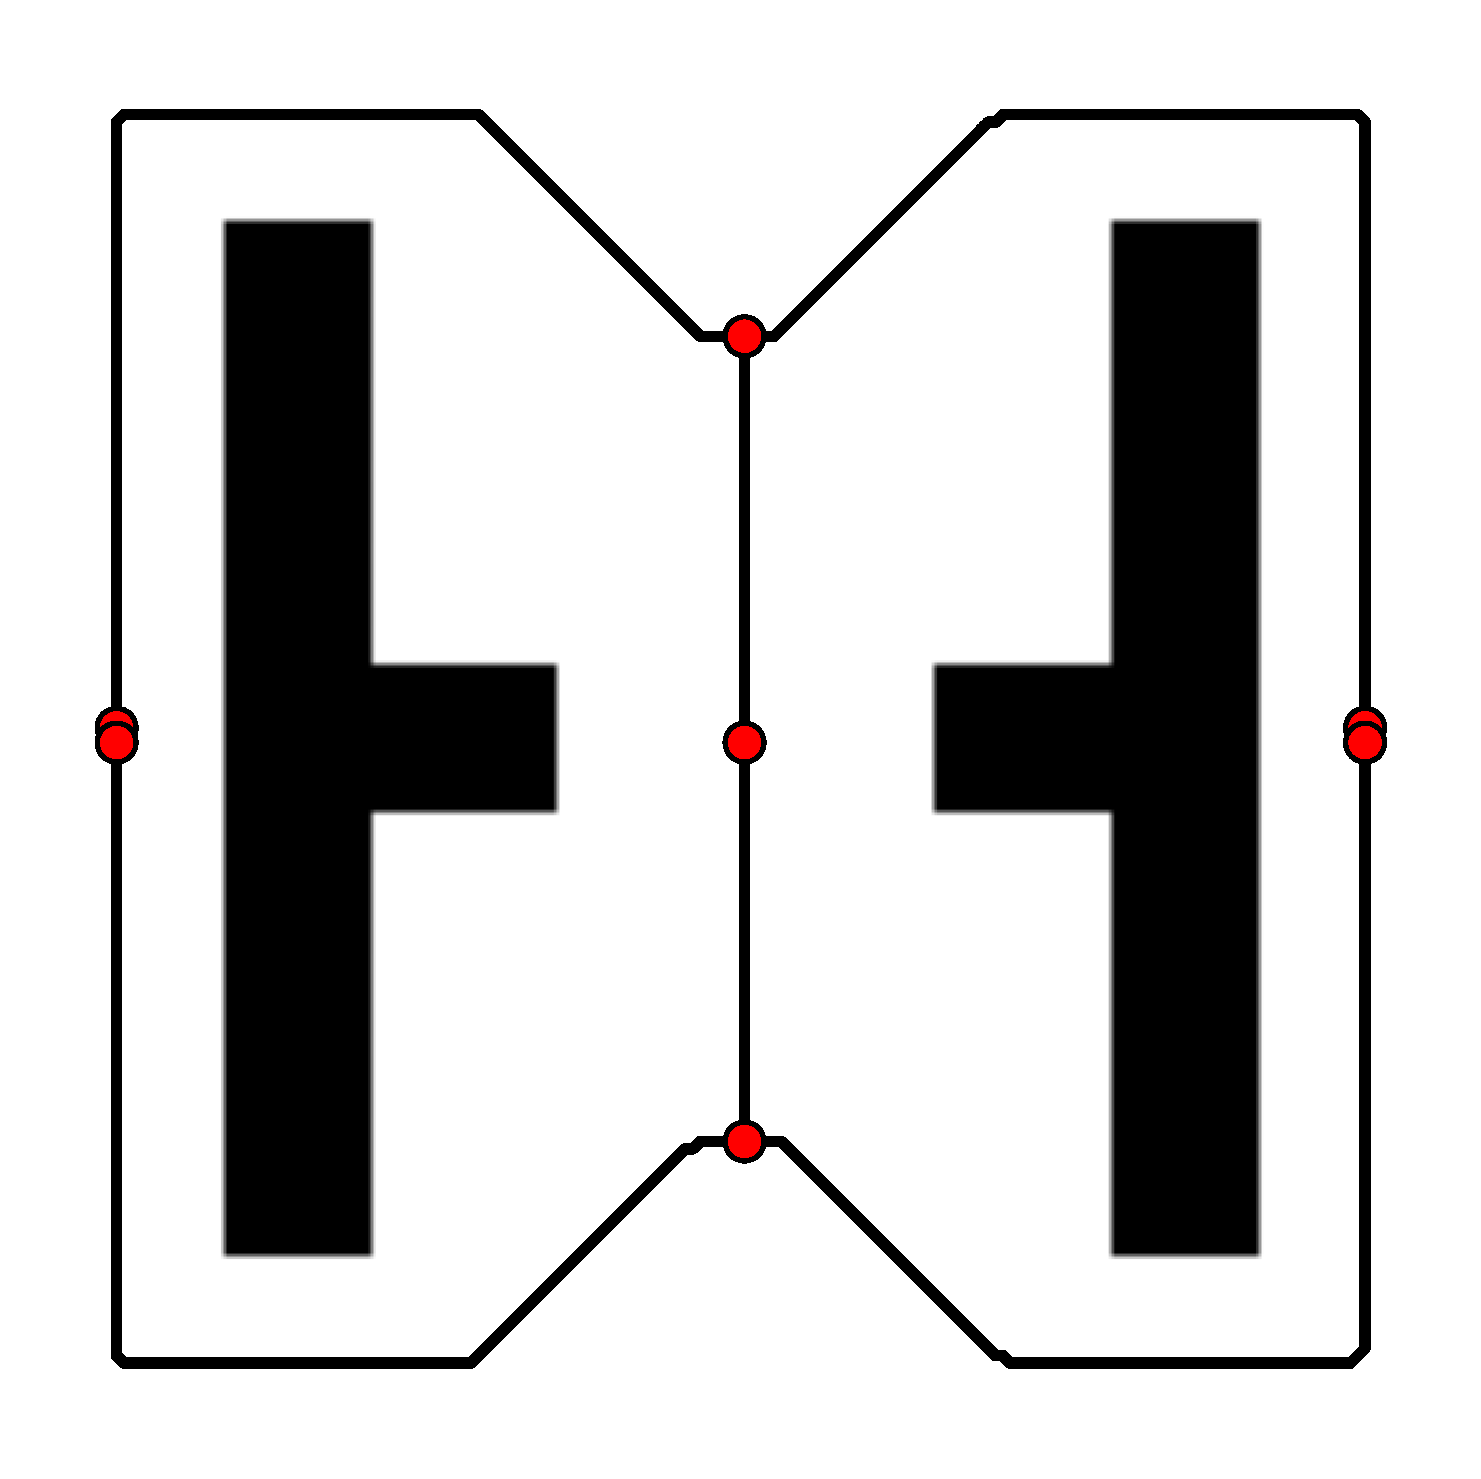
\includegraphics[width=0.24\linewidth]{figs/bars_david}
    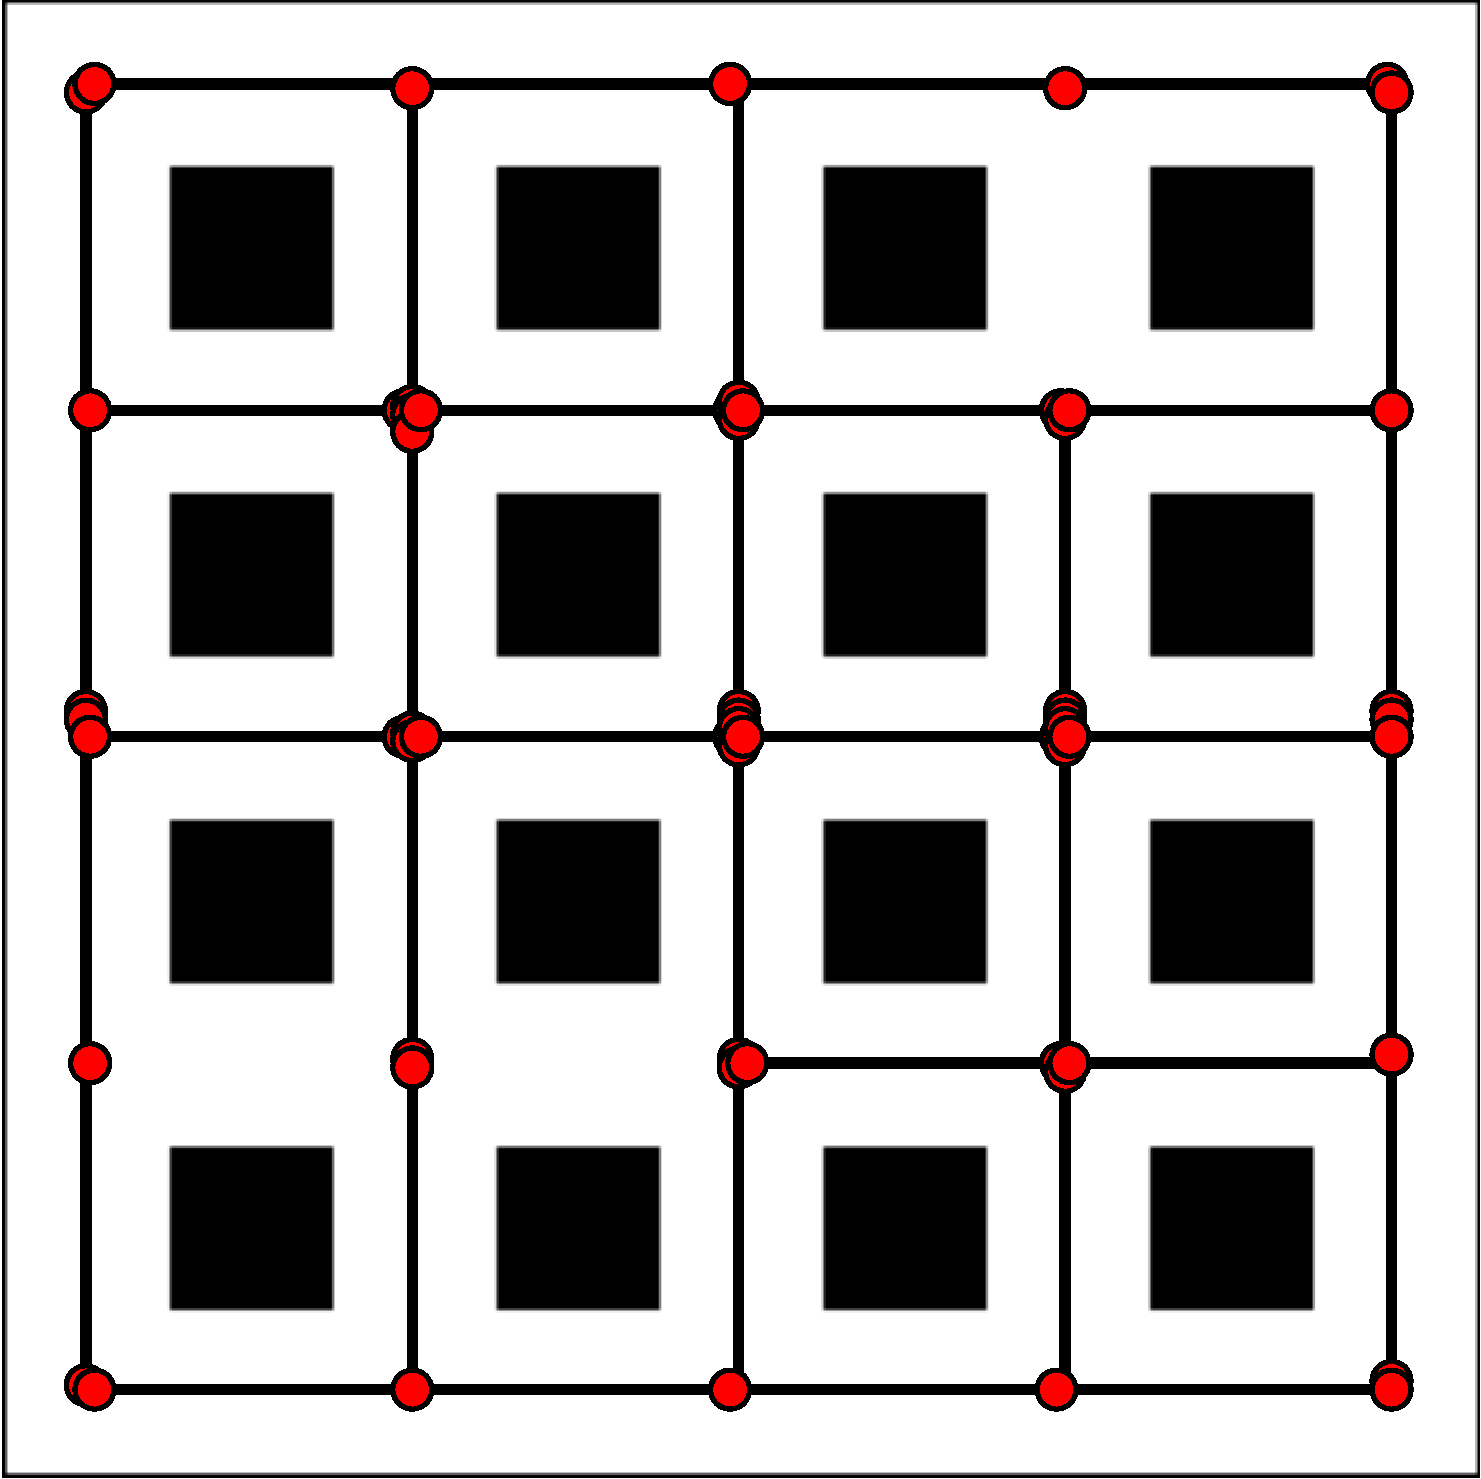
\includegraphics[width=0.24\linewidth]{figs/Grelha4_david}
    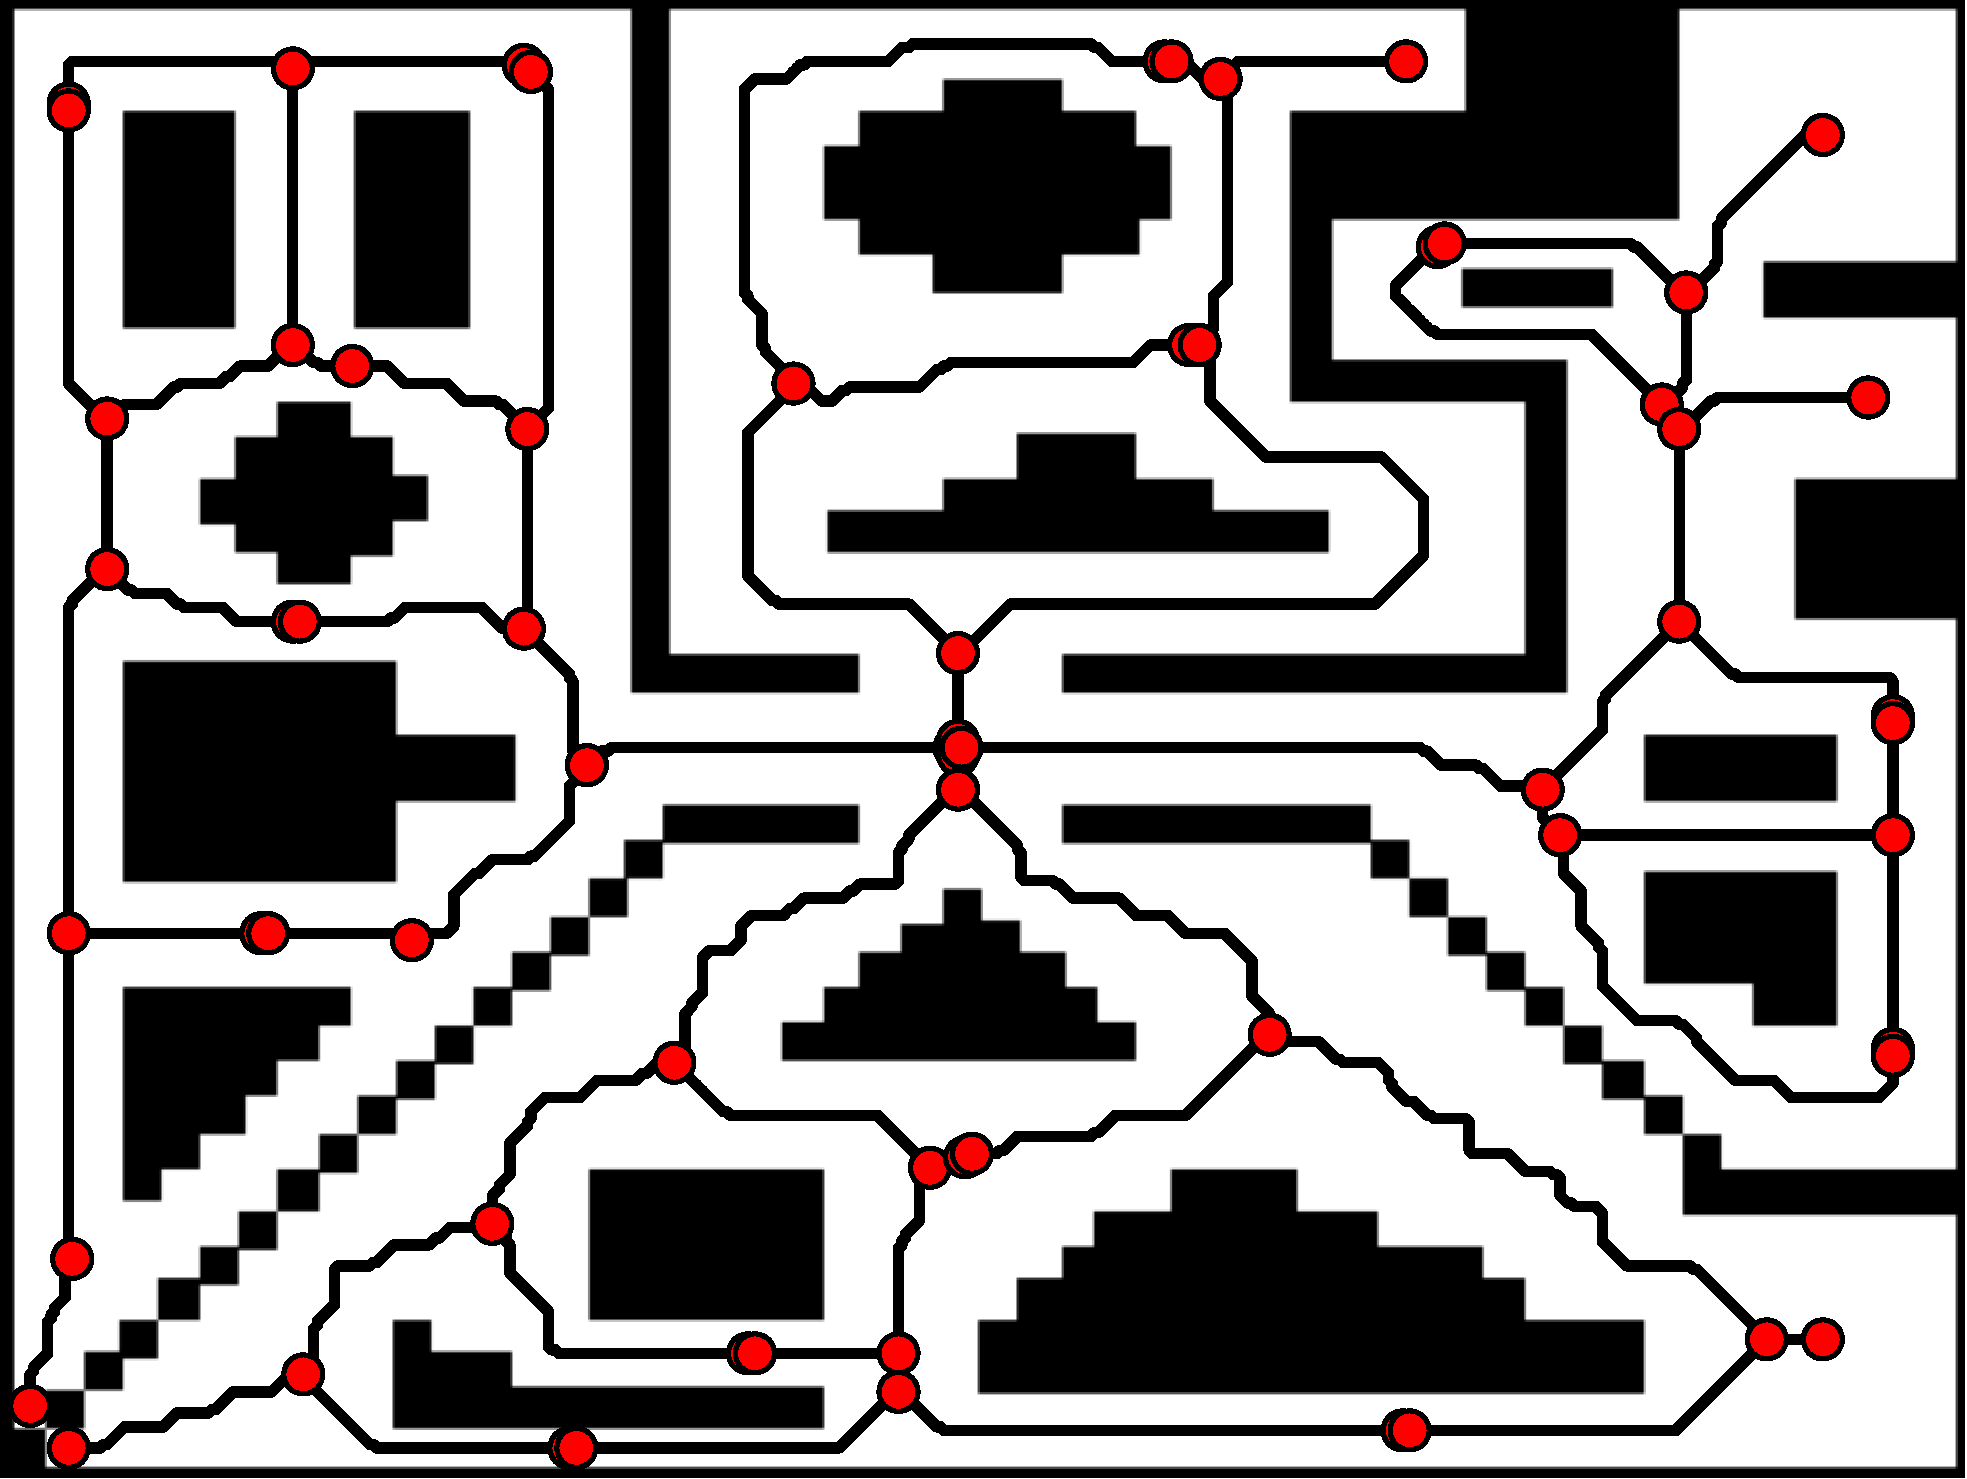
\includegraphics[width=0.32\linewidth]{figs/strongly_connected_david}

    \label{fig:david}
    \caption{The topological graph extracted using the algorithm by Portugal
        and Rocha shown in \cite{david}}
\end{figure*}

\section{Experimental Results}

\begin{figure}
    \centering
    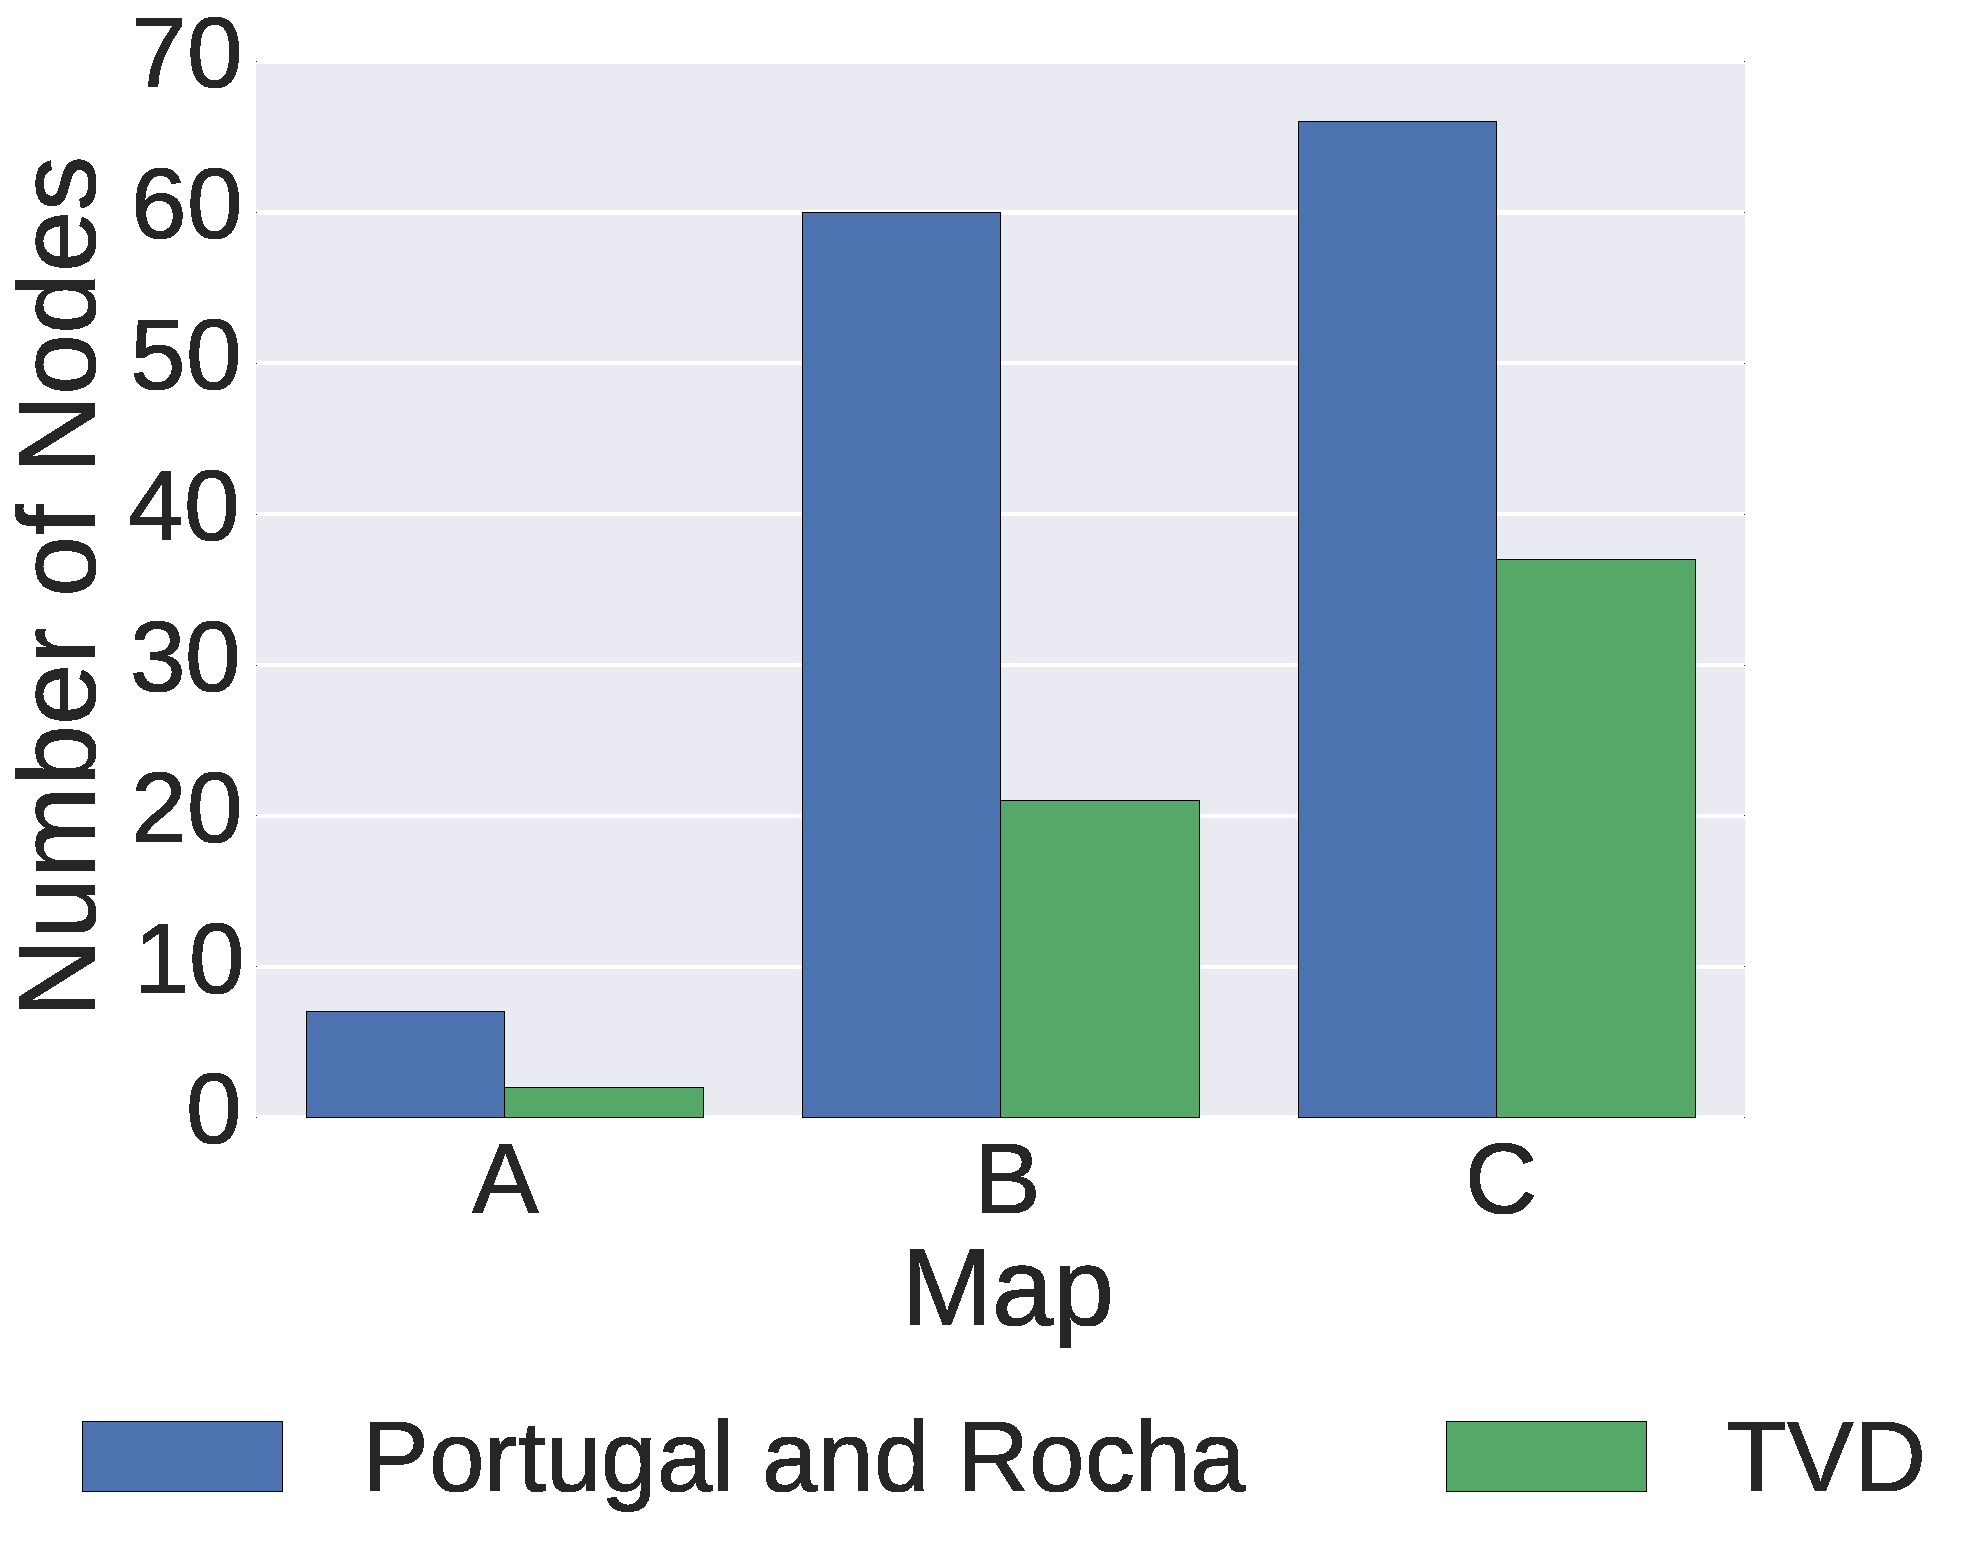
\includegraphics[width=\linewidth]{figs/number_of_nodes}
    \label{fig:compare}
    \caption{Plot comparing the number of nodes generated using the
        proposed $\Function{TVD}$ algorithm and the algorithm developed
        in \cite{david}}
\end{figure}

\section{Conclusion}

% \section{Graph Partitioning}
% 
% \begin{algorithm}[ht]
%     \caption{$\Function{Partition}(G, k)$}
%     \algorithmicrequire{
%         \begin{itemize}
%             \item $G = (V, E)$: Graph representing the topological
%                     connectivity of the environment
%             \item $k$: Desired number of subgraphs
%         \end{itemize}}
%     \algorithmicensure{
%         \begin{itemize}
%             \item A multi-graph where each vertex represents a partitioned
%                 subgraph and each edge represents a path between subgraphs
%         \end{itemize}}
% 
%     \label{algo:partition}
%     \begin{algorithmic}[1]
%         \setcounter{ALC@line}{0}
%         \vspace*{1mm}
%         \STATE $D \leftarrow \Function{FloydWarshall}(G)$
%         \STATE $L = (\mathcal{V}, \mathcal{E}) \leftarrow \Function{AgglomerativeClustering}_k(G, D)$
%         \STATE $H = (V', E') \leftarrow \Function{MultiDiGraph}()$
%         \FOR{$(p, q) \in E$}
%             \IF{$L_p \neq L_q$}
%                 \STATE $E' \leftarrow E' \cup (L_p, L_q, \Pi_G(p, q))$
%                 % \STATE $c \leftarrow \Function$
%                 \STATE $\Pi_{p \rightarrow c}, \Pi_{c \rightarrow q} \leftarrow \Function{SplitPath}(\Pi_G(p, q))$
%                 \STATE $\mathcal{E}_p \leftarrow (p, c, \Pi_{p \rightarrow c}),
%                 \mathcal{E}_p \leftarrow (c, p, \Pi_{c \rightarrow p})$
%                 \STATE $\mathcal{E}_q \leftarrow (c, q, \Pi_{c \rightarrow q}),
%                 \mathcal{E}_q \leftarrow (q, c, \Pi_{q \rightarrow c})$
%             \ENDIF
%         \ENDFOR
%         \RETURN $H$
%     \end{algorithmic}
% \end{algorithm}

\bibliographystyle{IEEEtran}
\bibliography{mp}

\end{document}

